
\section{Experiments}
\label{sec:experiments}

In this section, we empirically evaluate \model on image generation in terms of quality, efficiency and flexibility.
In \ref{ssec:class_conditional_synthesis}, we evaluate \model on the standard class-conditional image generation tasks on ImageNet~\cite{deng2009imagenet} 256$\times$256 and 512$\times$512.
In~\ref{ssec:applications}, we show \model's versatility by demonstrating its performance on three image editing tasks, image inpainting, outpainting, and editing. In~\ref{ssec:ablation}, we verify the necessity of our design of mask scheduling. We will release the code and model for reproducible research.


\subsection{Experimental Setup}
\label{ssec:architecture}

For each dataset, we only train a single autoencoder, decoder, and codebook with 1024 tokens on cropped 256x256 images for all the experiments. The image is always compressed by a fixed factor of 16, \ie from $H\times W$ to a grid of tokens in the size of $h \times w$, where $h$=$H / 16$ and $w$=$W/16$. We find that this autoencoder, together with the codebook, can be reused to synthesize 512$\times$512 images.

All models in this work have the same configuration: 24 layers, 8 attention heads, 768 embedding dimensions and 3072 hidden dimensions. Our models use learnable positional embedding\cite{Vaswani17attention}, LayerNorm\cite{ba2016layer}, and truncated normal initialization (stddev=$0.02$). We employ the following training hyperparameters: label smoothing=$0.1$, dropout rate=$0.1$, Adam optimizer~\cite{kingma2014adam} with $\beta_{1}$=$0.9$ and $\beta_{2}$=$0.96$. We use RandomResizeAndCrop for data augmentation. All models are trained on 4x4 TPU devices with a batch size of 256. ImageNet models are trained for 300 epochs while the Places2 model is trained for 200 epochs. 

\subsection{Class-conditional Image Synthesis}
\label{ssec:class_conditional_synthesis}

We evaluate the performance of our model on class-conditional image synthesis on ImageNet 256$\times$256 and 512$\times$512. Our main results are summarized in Table~\ref{tab:maintable}.

\noindent\textbf{Quality.}
On ImageNet 256$\times$256, without any special sampling strategies such as beam-search, top-k or nucleus sampling heuristics~\cite{holtzman2019nucleus} or classifier guidance~\cite{Razavi19vqvae2}, we significantly outperform VQGAN~\cite{Esser21vqgan} in both Fr\'{e}chet Inception Distance (FID)~\cite{FID} ($\bestfid$ vs $15.78$) and Inception Score (IS) ($\bestis$ vs $78.3$). We also report the results with classifier-based rejection sampling in the appendix \ref{sec:supp_diversity_comparison}. 

%
We also train a VQGAN baseline with the same tokenizer and hyperparameters as \model's in order to further highlight the difference between bi-directional and uni-directional transformers, and find that on both resolutions, \model still outperforms our implemented baseline by a significant margin. 

Furthermore, \model improves BigGAN's FIDs on both resolutions, achieving a new state-of-the-art on 512$\times$512 with an FID of $7.32$.

\begin{figure}[!t]
	\centering
	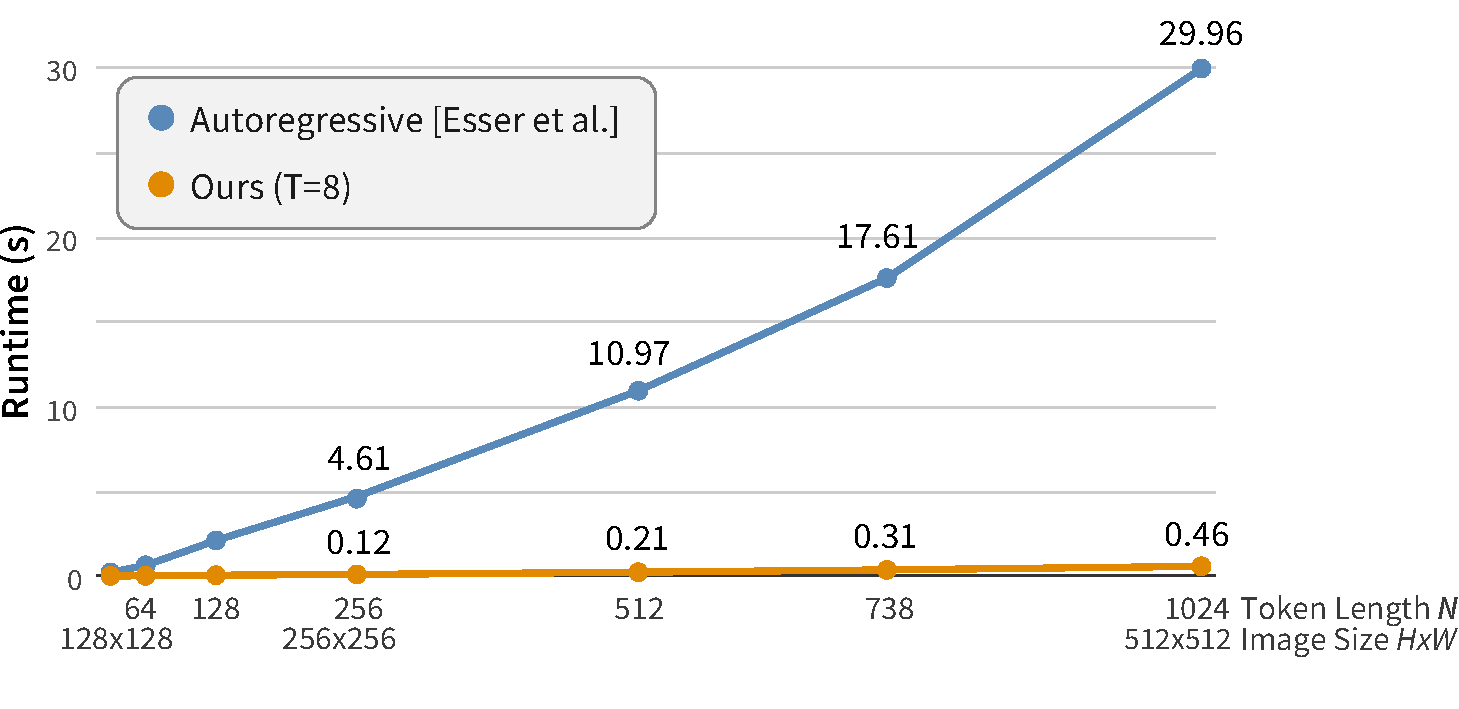
\includegraphics[width=1.\linewidth]{figures/runtime.pdf}
	\vspace{-5mm}
	\caption{\textbf{Transformer wall-clock runtime comparison between VQGAN\cite{Esser21vqgan} and ours.} All results are run on a single GPU. }
	\label{fig:speed}
 	\vspace{-4mm}
\end{figure}
{
\newcolumntype{N}{@{}m{0pt}@{}}

\begin{table*}[h]
\small
    \centering
    {\small
    \begin{tabular}{lc ccc ccc ccc cc}
    \toprule
     {Model} & 
    
     & {FID}  $\downarrow$ & {IS}  $\uparrow$ & 
     &  {Prec}  $\uparrow$ & {Rec}   $\uparrow$ &
     
     &{\# params} & {\# steps} &
     
     & \multicolumn{2}{c}{{CAS $\times 100$} $\uparrow$}  
     \\
     \cline{12-13}
    &&  && & &&& & && {Top-1 (76.6)} & {Top-5 (93.1)} \\[-7pt]
    \textbf{ImageNet 256$\times$256} && &&& &&& &&& &
    \\[-2pt]
    \midrule
    
    DCTransformer~\cite{nash2021generating} $^\square$ &
    & 36.51 & n/a &
    & 0.36 & \textbf{0.67} &
    & 738M & $>$1024 &   & &
     \\ 
    
    BigGAN-deep~\cite{biggan}  & %, 1.0 trunc. &
    & 6.95 & \bfseries{198.2} &
    & \textbf{0.87} & 0.28 &
    & 160M & 1 & & 43.99 &67.89
    \\
    
    % Improved DDPM~\cite{nichol2021improved} &
    % & 31.5 &   &
    % & ?0.70 & ?0.62 &
    % &  & &
    % & 270M & 250 \\
    Improved DDPM~\cite{nichol2021improved}$^\square$  &
    & 12.26 & n/a  &
    & 0.70 & 0.62 &
     & 280M & 250  &  &  & \\
    
    ADM~\cite{dhariwal2021diffusion}$^\square$   & 
    & 10.94 & 101.0  &
    & 0.69 & 0.63 &
    & 554M & 250 &  &  & \\
    
    % ADM-G, 1.0 guid. & 
    % & 4.59 & 186.7  &
    % & ?0.69 & ?0.63 &
    % &  &  &
    % & 554M & 250  %554M + 54M classfier
    % \\

    
    VQVAE-2~\cite{Razavi19vqvae2}$^\square$ &
    & 31.11 & $\sim$45 &
    & 0.36 & 0.57 &
    & 13.5B$^\dagger$ & 5120 & & 54.83 & 77.59 \\
   % \midrule
   % \bfseries{\model Baseline} && 18.98 & 192.52 && ? & ? && ?? & ?? \\
    \midrule
    VQGAN~\cite{Esser21vqgan}$^\square$ &
    
    & 15.78 & 78.3 &
    & n/a & n/a &
    & 1.4B & 256 &  &  &
    \\
 
    VQGAN$^\ast$ &
    & 18.65 & 80.4 &
    & 0.78 & 0.26 &
    & 227M & 256 & 
    & 53.10 & 76.18
     \\   
    % VQ-GAN, 0.05 RS &
    % & 1.4B +  & 5120 &
    % & 5.20 & 380.3 &
    % % & ? & ? &
    % &  & \\
%     \bfseries{\model-Linear} &
    
%     &  &  &
%     &  &  &
%   & 227M  & 16 &
%      & &
   
    \bfseries{\model (Ours)} &
    
    & \bfseries{\bestfid} & \bestis &
    & 0.80 & 0.51 &
   & 227M  & \textit{8} &
   & \bfseries{63.14} & \bfseries{84.45}
    \\
%    & & \textbf{5.14} & 184.0 & &  0.78 & 0.52 & & 227M & \textit{64} &
%    & &  \\
    % 227M + 54M
    % \bfseries{Ours, 0.05 RS} &
    % & +  &  &
    % & 5.90 & 152.9 &
    % % & ? & ? &
    % &  &  \\

   
    % Validation &
    % &- & - &
    % & 1.62 & 234.0  &
    % % & ? & ? &
    % &  73.09 &  91.47 \\
    \bottomrule
    \\[-4pt]
    \textbf{ImageNet 512$\times$512} && &&& &&& &&& &\\[-2pt]
    \midrule
    
     BigGAN-deep~\cite{biggan} & & 8.43 & \bfseries{232.5} & & \textbf{0.88} & 0.29 &
     &160M&1& 
     &44.02&68.22\\
     
     ADM~\cite{dhariwal2021diffusion}$^\square$ & & 23.24 & 58.06  &&0.73& \textbf{0.60} & 
     &559M&250&
     && \\
    %  ADM, 1.0 guid. & 7.72 & & 0.87 & 0.42  \\
     \midrule
     VQGAN$^\ast$ & & 26.52 & 66.8 &
     & 0.73 & 0.31 &
      & 227M &1024 &
     &51.29&74.24 \\
     \bfseries{\model (Ours)} & & \bfseries{\bestfidhighres} & 156.0 & &  0.78 & 0.50 & & 227M &\textit{12}&
     &\textbf{63.43} & \textbf{84.79}  \\
    %  & & \bfseries{5.94} & 169.4 & & 0.77 & 0.48 & & 227M & \textit{256} &
    %  & &  \\
     % \bfseries{Ours}, 0.5 RS & ? & ? & &  \\
    \bottomrule
    
    \end{tabular}
    }
    \vspace{-5pt}
    \caption{Quantitative comparison with state-of-the-art generative models on ImageNet 256$\times$256 and 512$\times$512. 
    %
    \footnotesize{``\# steps” refers to the number of neural network runs needed to generate a sample.  $^\ast$ denotes the model we train with the same architecture and setup with ours; $^\square$ denotes values taken from prior publications;  $^\dagger$ estimated based on the pytorch implementation~\cite{pytorch2020vqvae2}.} 
    }
    % $^\blackdiamond$ indicates classifiers trained with data augmentation Randaugment~\cite{cubuk2019randaugment};
    \label{tab:maintable}
    % On average 10-15ms per step

\end{table*}


% \begin{table}[h]
% \small
%     \centering
%     {\small
%     \begin{tabular}{lcccc}
%     \toprule    
%     \bfseries{Model} & \bfseries{FID}  $\downarrow$ & \bfseries{IS}  $\uparrow$ & \bfseries{Prec} $\uparrow$  & \bfseries{Rec} $\uparrow$ \\ \midrule
    %  BigGAN-deep~\cite{biggan} & 8.43 & \bfseries{232.5} & 0.88 & 0.29 \\
    %  ADM~\cite{dhariwal2021diffusion} & 23.24 & &0.73& 0.60  \\
    % %  ADM, 1.0 guid. & 7.72 & & 0.87 & 0.42  \\
    % % \midrule
    %  VQGAN$^\ast$ & 25.36 & 102.8 &&  \\
    %  \bfseries{Ours} & \bfseries{\bestfidhighres} & 156 & &  \\
    %  % \bfseries{Ours}, 0.5 RS & ? & ? & &  \\
    % \bottomrule
%     \end{tabular}
%     }
%     % \vspace*{0.35cm}
%     \caption{Quantitative comparison with state-of-the-art generative models on ImageNet $512 \times 512$. $^\ast$ denotes models we train with the same architecture and setup with ours. 
%     \todo{rerun with the same codebook} }
%     \label{tab:imagenet512}
% \vspace{-.2cm}
% \end{table}


% \begin{table}[h]
% \small
%     \centering
%     {\small
%     \begin{tabular}{lc ccc ccc cc}
%     \toprule
%  Reconstruction &
%     &  & &
%     & 2.64 & 191.4 &
%     % & ? & ? &
%     & ? & ? \\
%         \bottomrule
%     \end{tabular}
%     }
%     \caption{Reconstruction}
%     \label{tab:reconstruction}
% \vspace{-.2cm}
% \end{table}
\newcommand{\tmpwidth}{0.31\linewidth}

\begin{figure*}[!ht]
    \centering
    \begin{tabular}{c c c}
     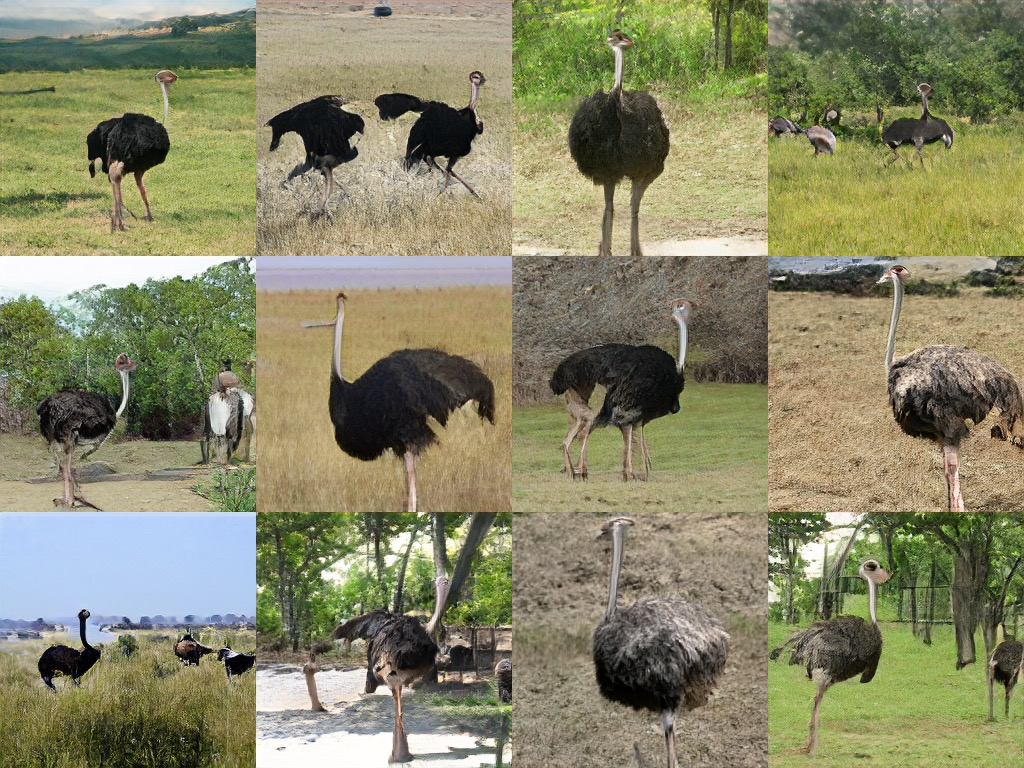
\includegraphics[ width=\tmpwidth]{figures/diversity/009_biggan_trun1.jpeg} & \hspace{-3mm}
    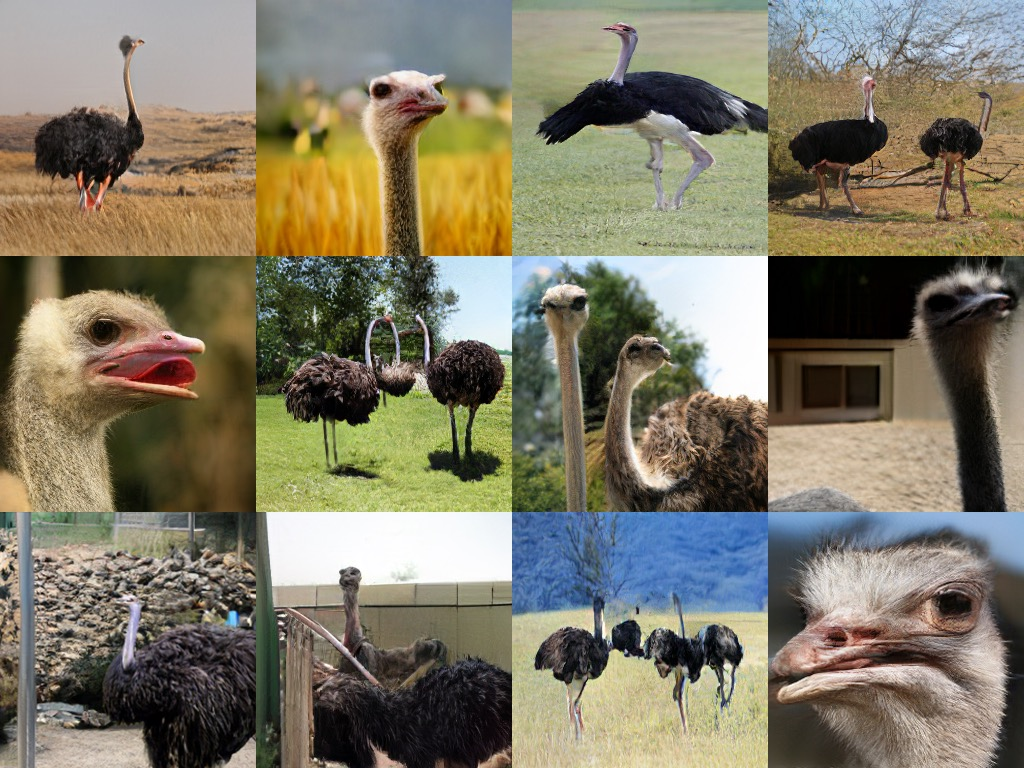
\includegraphics[ width=\tmpwidth]{figures/diversity/009_ours.jpeg} & \hspace{-3mm}
    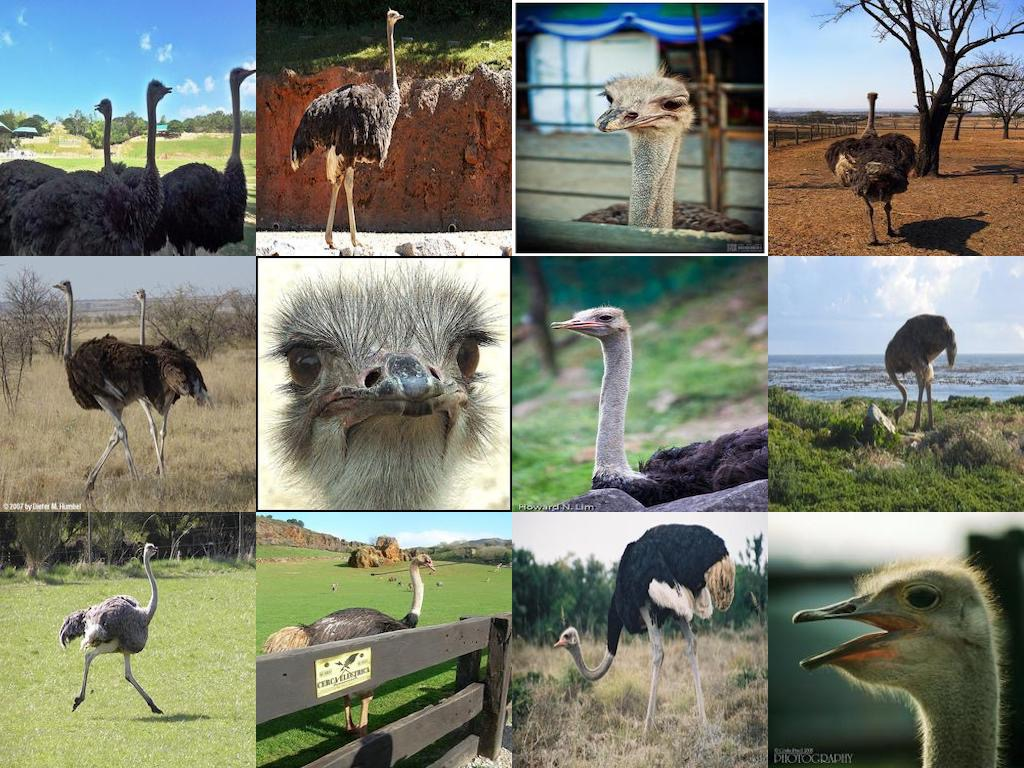
\includegraphics[ width=\tmpwidth]{figures/diversity/009_gt.jpeg} \\ 
    
    % \includegraphics[ width=\tmpwidth]{figures/diversity/130_biggan_trun1.jpeg} & \hspace{-3mm}
    % \includegraphics[ width=\tmpwidth]{figures/diversity/130_ours.jpeg} & \hspace{-3mm}
    % \includegraphics[ width=\tmpwidth]{figures/diversity/130_gt.jpeg} \\ 
 
    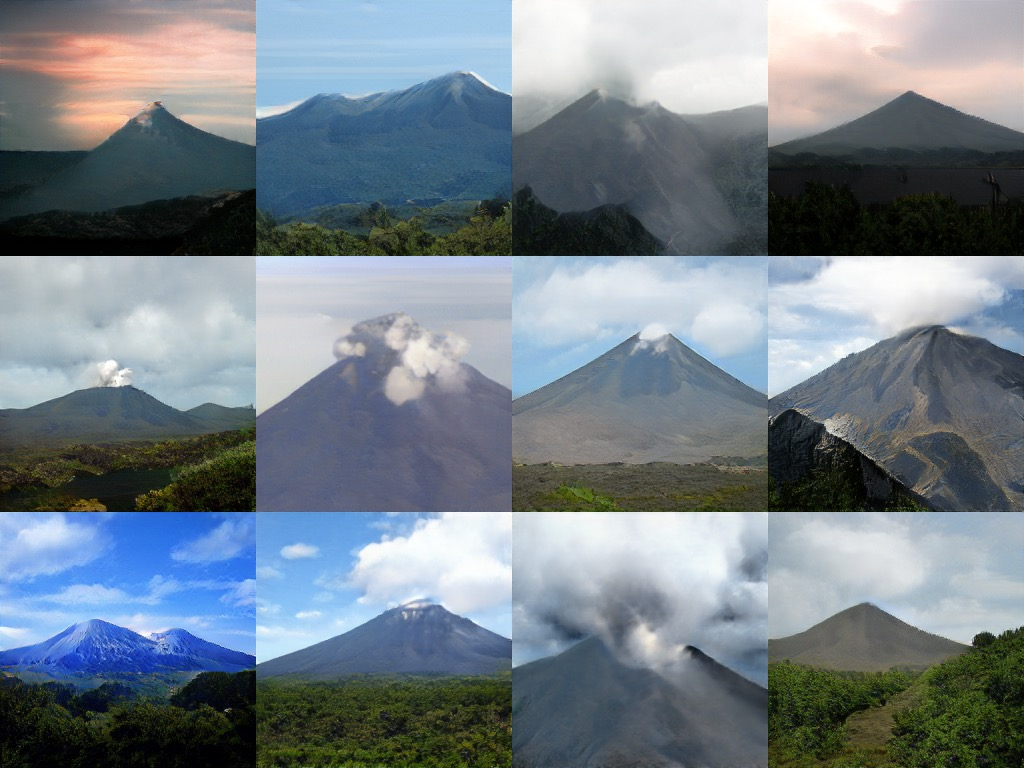
\includegraphics[ width=\tmpwidth]{figures/diversity/980_biggan_trun1.jpeg} & \hspace{-3mm}
    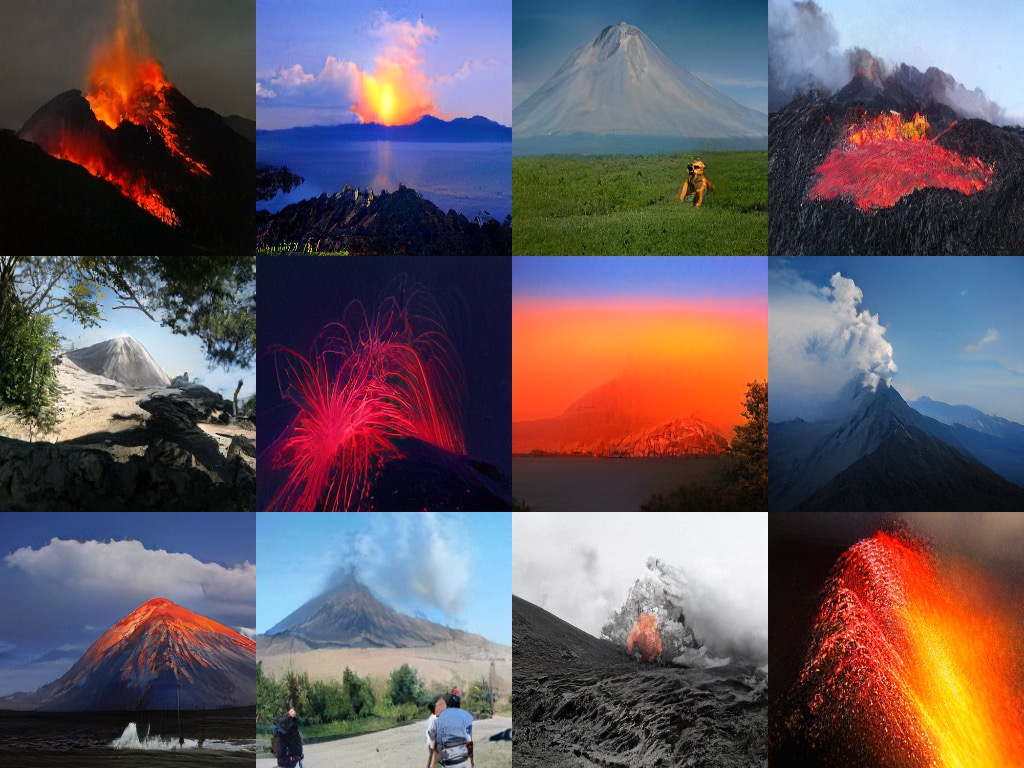
\includegraphics[ width=\tmpwidth]{figures/diversity/980_ours1.jpeg} & \hspace{-3mm}
    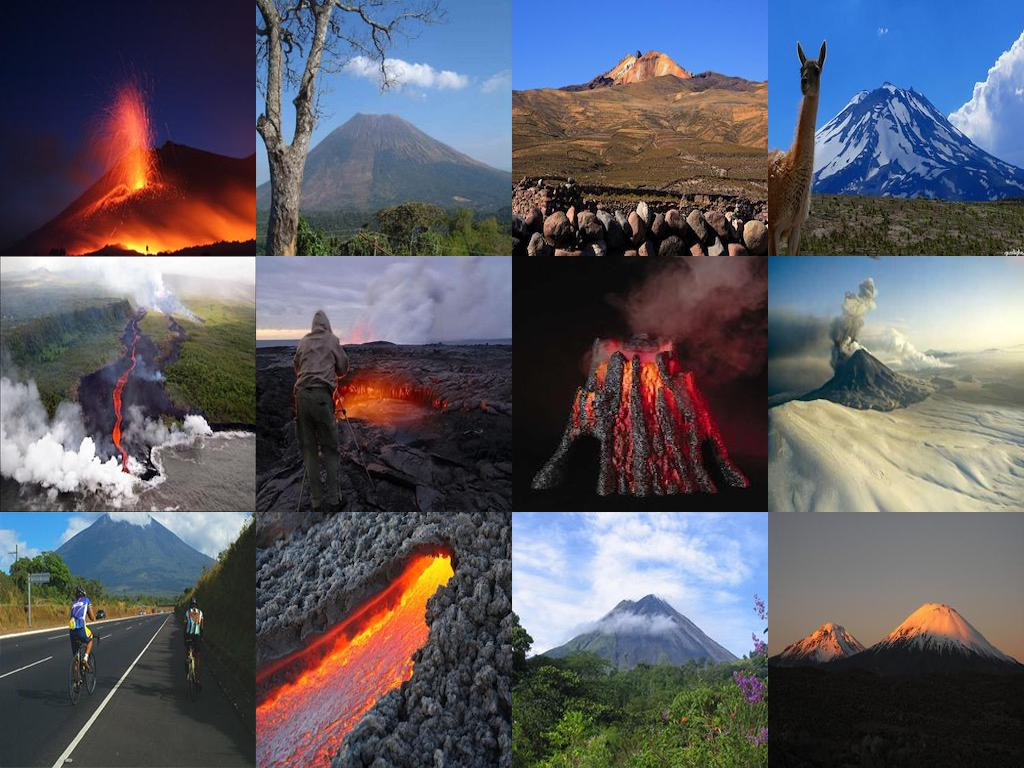
\includegraphics[ width=\tmpwidth]{figures/diversity/980_gt.jpeg} \\
    
    % \includegraphics[ width=\tmpwidth]{figures/diversity/145_biggan_trun1.jpeg} & \hspace{-3mm}
    % \includegraphics[ width=\tmpwidth]{figures/diversity/145_ours.jpeg} & \hspace{-3mm}
    % \includegraphics[ width=\tmpwidth]{figures/diversity/145_gt.jpeg} \\
    
    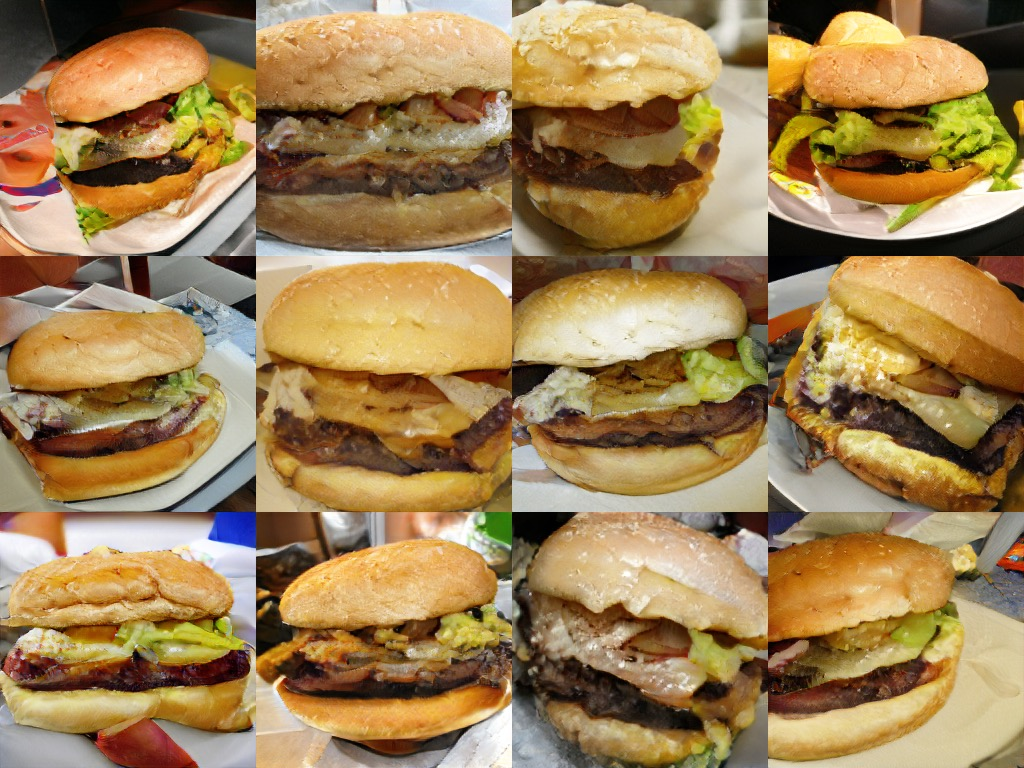
\includegraphics[ width=\tmpwidth]{figures/diversity/933_biggan_trun1.jpeg} & \hspace{-3mm}
    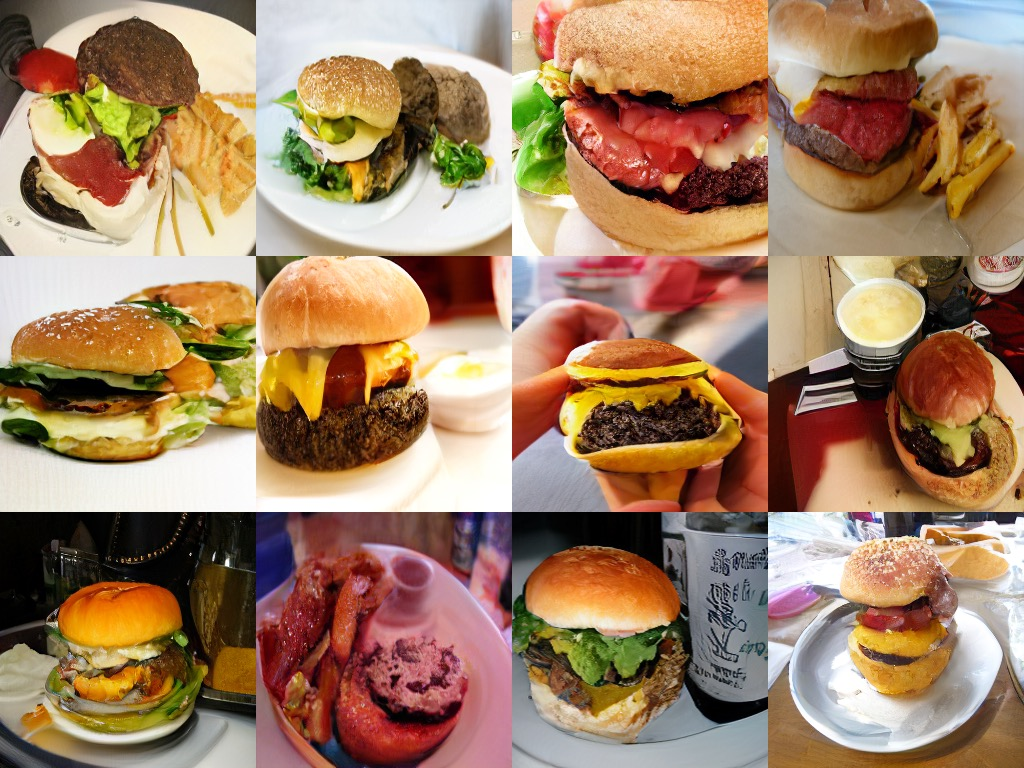
\includegraphics[ width=\tmpwidth]{figures/diversity/933_ours.jpeg} & \hspace{-3mm}
    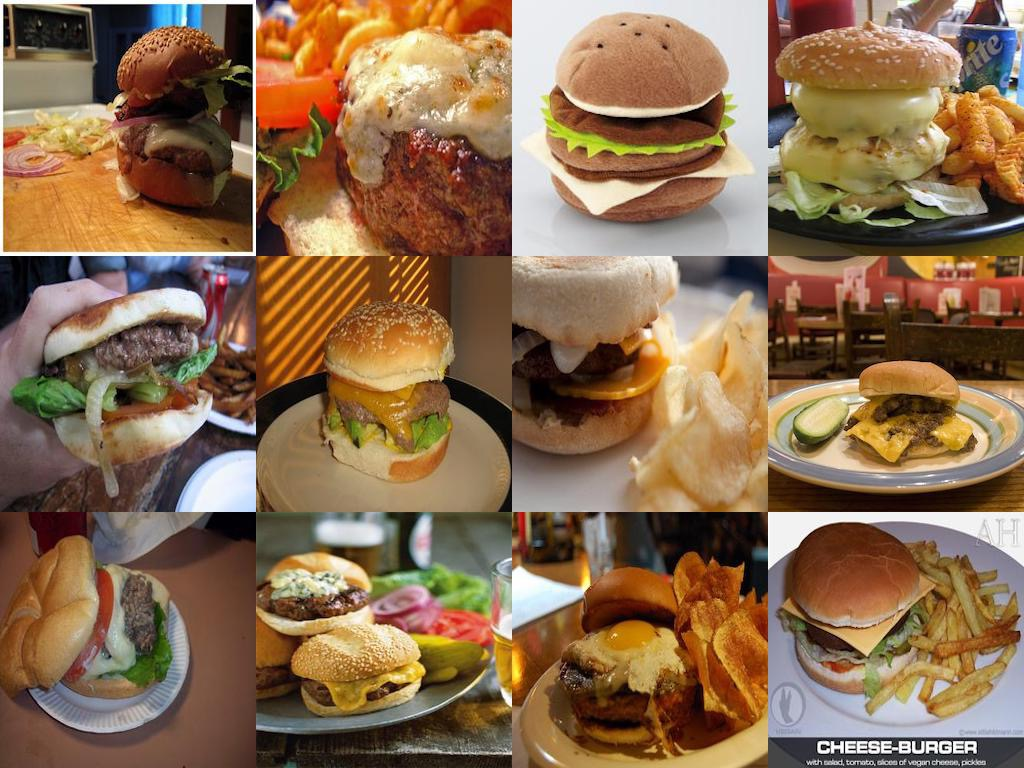
\includegraphics[ width=\tmpwidth]{figures/diversity/933_gt.jpeg} \\     

    % \includegraphics[ width=\tmpwidth]{figures/diversity/000_biggan_trun1.jpeg} & \hspace{-3mm}
    % \includegraphics[ width=\tmpwidth]{figures/diversity/000_ours1.jpeg} & \hspace{-3mm}
    % \includegraphics[ width=\tmpwidth]{figures/diversity/000_gt.jpeg} \\   
    
    BigGAN-deep (FID=$6.95$) & \model (FID=\bestfid) & Training Set \\
    \end{tabular}
    \vspace{-2mm}
    \caption{Sample Diversity Comparison between our proposed method \model and BigGAN-deep~\cite{biggan} on ImageNet 256$\times$256. 
    %BigGAN was sampled with $1.0$ truncation to yield the maximum diversity. In contrast to BigGAN's samples, our proposed method generate more diverse samples such as varied lighting, poses, scales and context, which are visually closer to the training set.
    The class ids of the samples from top to bottom  are {\footnotesize{ \texttt{009}}, \footnotesize{\texttt{980}} and \footnotesize{\texttt{993}}} respectively. Please refer to appendix for more comparisons.}
    \vspace{-6mm}
    \label{fig:diversity}
\end{figure*}
}

\newcommand{\tmpwidth}{0.23\linewidth}
\setlength{\tabcolsep}{1pt}
\begin{figure}[!t]
    \centering
    \begin{tabular}{c c c c }

	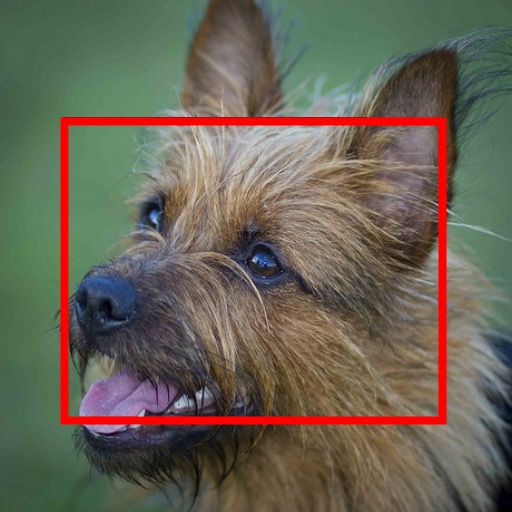
\includegraphics[width=\tmpwidth]{figures/editing/000193_to282_0006_input.jpeg} &
	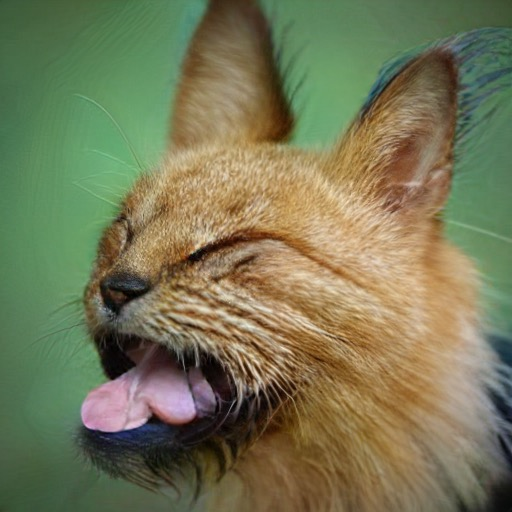
\includegraphics[width=\tmpwidth]{figures/editing/000193_to282_0006_output.jpeg}&
	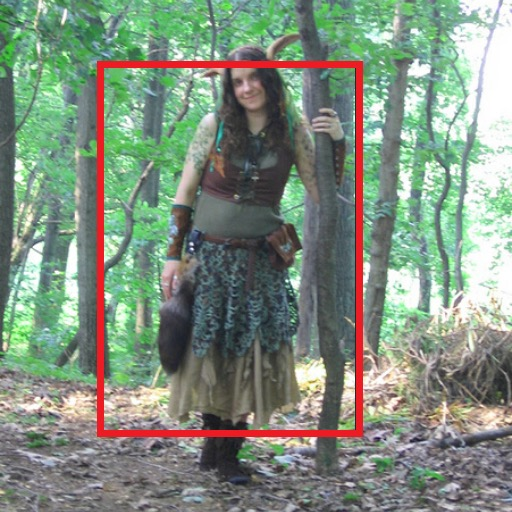
\includegraphics[width=\tmpwidth]{figures/editing/000689_to282_0000_input.jpeg} &
	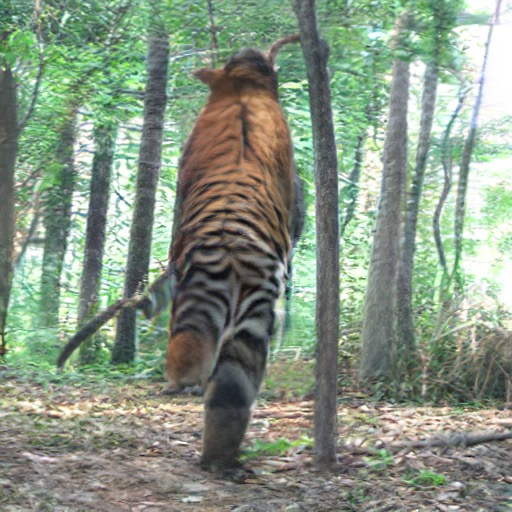
\includegraphics[width=\tmpwidth]{figures/editing/000689_to282_0000_output.jpeg} 
	\\
	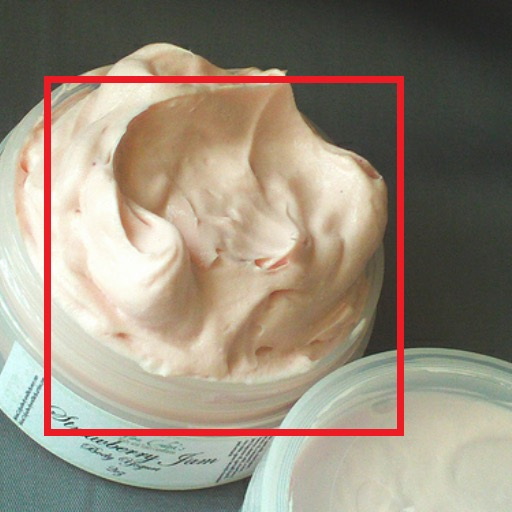
\includegraphics[width=\tmpwidth]{figures/editing/000838_to282_0004_input.jpeg} &
	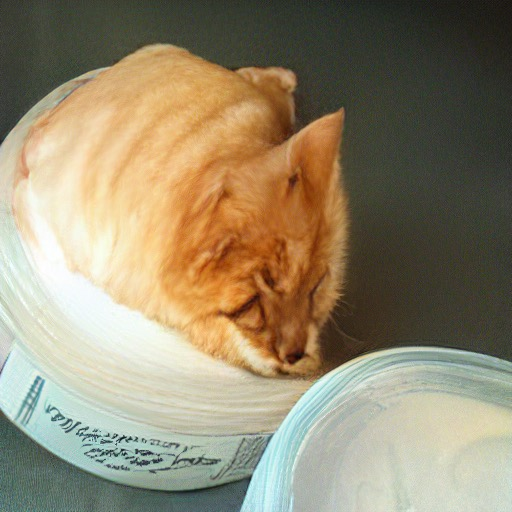
\includegraphics[width=\tmpwidth]{figures/editing/000838_to282_0004_output.jpeg} &
	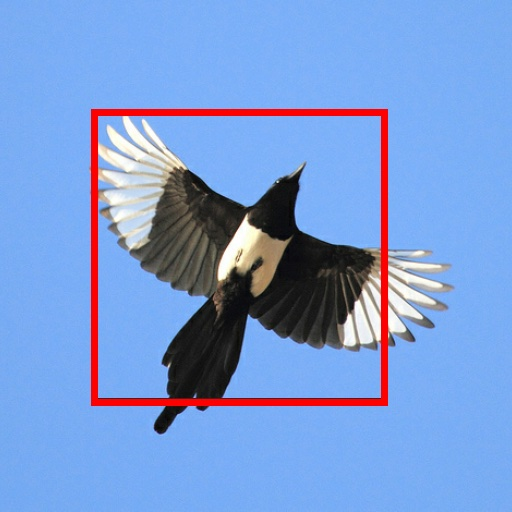
\includegraphics[width=\tmpwidth]{figures/editing/000018_to282_0002_input.jpeg} &
	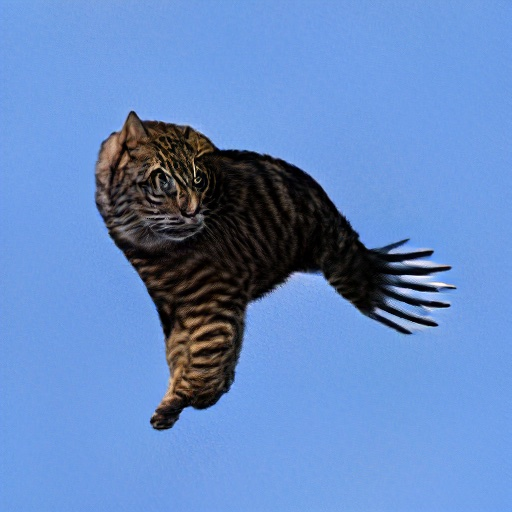
\includegraphics[width=\tmpwidth]{figures/editing/000018_to282_0000_output.jpeg} 
	
	\\
	
	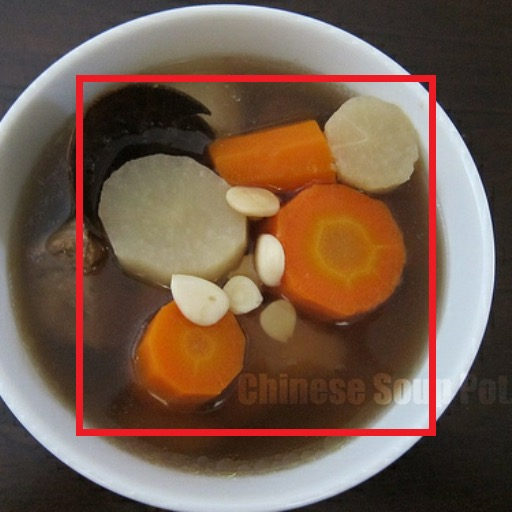
\includegraphics[width=\tmpwidth]{figures/editing/000809_to282_0002_input.jpeg} &
	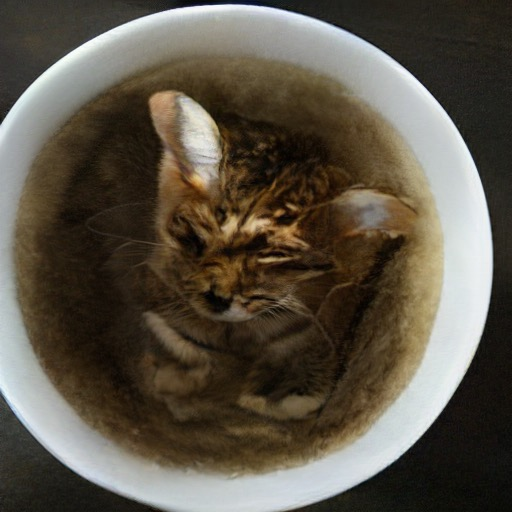
\includegraphics[width=\tmpwidth]{figures/editing/000809_to282_0002_output.jpeg} &
	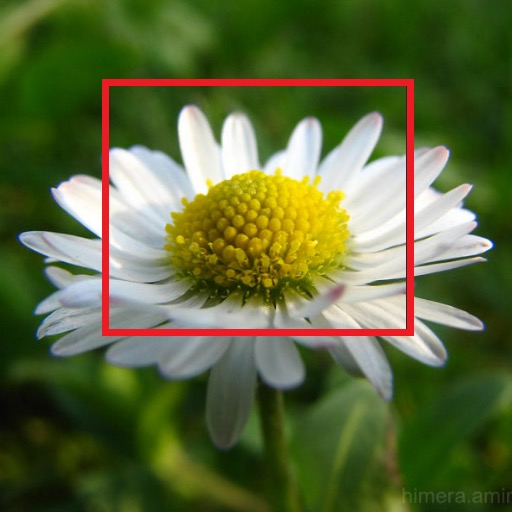
\includegraphics[width=\tmpwidth]{figures/editing/000985_to282_0000_0024_input.jpeg} &
    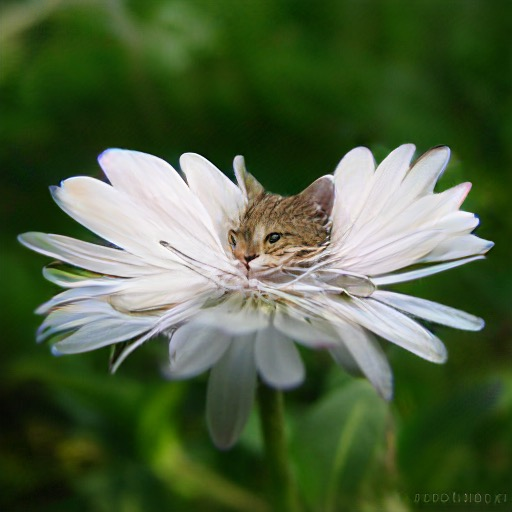
\includegraphics[width=\tmpwidth]{figures/editing/000985_to282_0000_0012_output.jpeg} 
    \\ 

    % \includegraphics[width=\tmpwidth]{figures/editing/000538_to282_0036_output.jpeg} &

    \end{tabular}
    \vspace{-3mm}
    \caption{\textbf{Class-conditional image editing.} Given input images on the left of each pair, and a target class "tiger cat", \model replaces the bounding boxed regions with tiger cats, suggesting the composition ability of our model. % The fact that the synthesized tiger cat blends in with the rest of the image seamlessly highlights the composition ability of our model. 
    }
    \vspace{-2mm}
    \label{fig:editing}
\end{figure}


\begin{figure}[!t]
    \centering
    \begin{tabular}{cccc}
  
    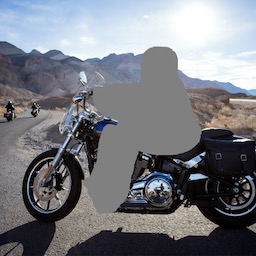
\includegraphics[width=\tmpwidth]{figures/uncrop/harley-davidson-xAHtaYIHlPI_input_0.jpeg}&

    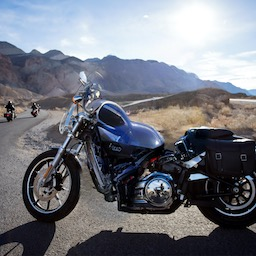
\includegraphics[width=\tmpwidth]{figures/uncrop/harley-davidson-xAHtaYIHlPI_output_12.jpeg}&
    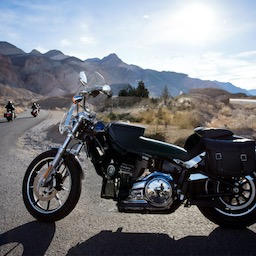
\includegraphics[width=\tmpwidth]{figures/uncrop/harley-davidson-xAHtaYIHlPI_output_03.jpeg}&
    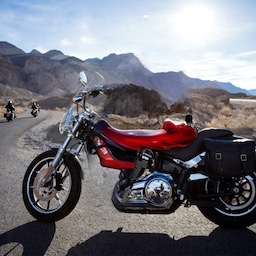
\includegraphics[width=\tmpwidth]{figures/uncrop/harley-davidson-xAHtaYIHlPI_output_06__.jpeg}

    \\
    
    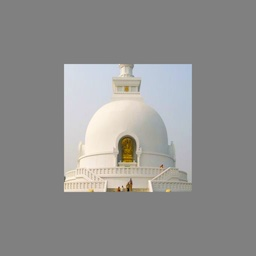
\includegraphics[width=\tmpwidth]{figures/uncrop/001704_input.jpeg}&
    % 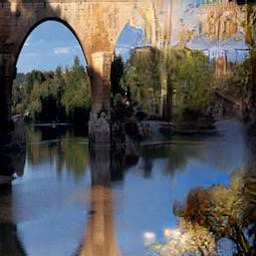
\includegraphics[width=\tmpwidth]{figures/uncrop/3101_boundless.jpeg}&
    % 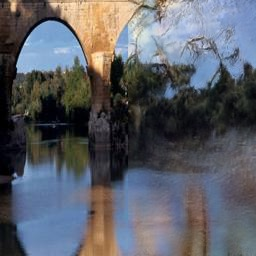
\includegraphics[width=\tmpwidth]{figures/uncrop/3101_inf.jpeg}&
    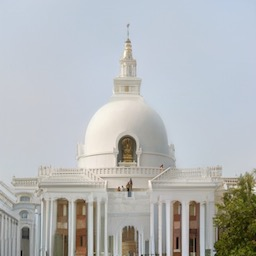
\includegraphics[width=\tmpwidth]{figures/uncrop/001704_ours_12.jpeg} &
    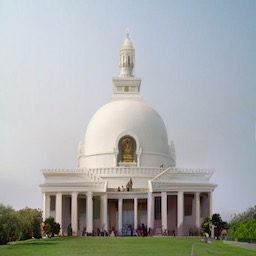
\includegraphics[width=\tmpwidth]{figures/uncrop/001704_ours_17.jpeg} &
    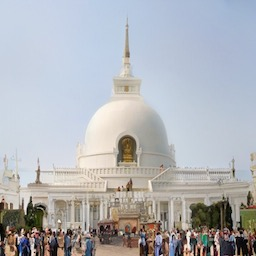
\includegraphics[width=\tmpwidth]{figures/uncrop/001704_ours_11.jpeg} 
    
    \\
    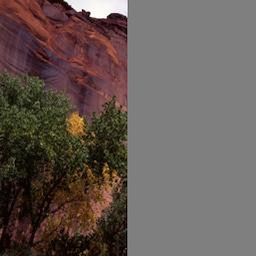
\includegraphics[width=\tmpwidth]{figures/uncrop/3996_input.jpeg}&
    %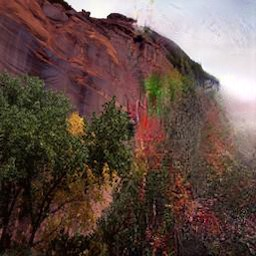
\includegraphics[width=\tmpwidth]{figures/uncrop/3996_boundless.jpeg}&
    % 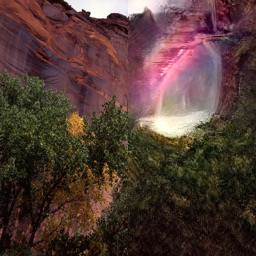
\includegraphics[width=\tmpwidth]{figures/uncrop/3996_inf.jpeg}&
    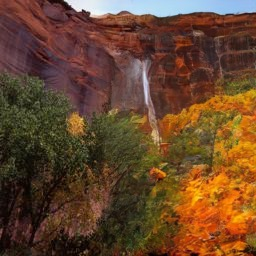
\includegraphics[width=\tmpwidth]{figures/uncrop/3996_output8.jpeg} &
    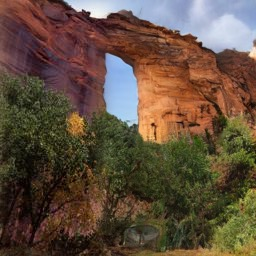
\includegraphics[width=\tmpwidth]{figures/uncrop/3996_output1.jpeg} &
    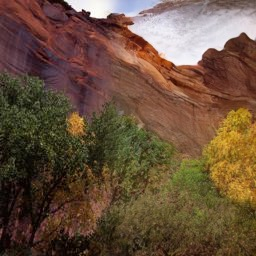
\includegraphics[width=\tmpwidth]{figures/uncrop/3996_output9.jpeg} 
    %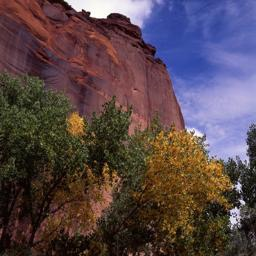
\includegraphics[width=\tmpwidth]{figures/uncrop/3996_gt.jpeg}
   \\
    \vspace{-1mm}
    Input  & \multicolumn{3}{c}{------ \model (Our Samples) ------} \\    
    % Input & DeepFill & HiFill  & \multicolumn{3}{c}{------ \model (Our Samples) ------} & Groundtruth \\    
    \end{tabular}
    \vspace{-1mm}
    \caption{\textbf{Inpainting and outpainting.} Given a single input image, \model synthesizes diverse results for inpainting (first row) and outpainting in different directions (last two rows).}
    \label{fig:uncrop_diversity}
    \vspace{-3mm}
\end{figure}

\setlength{\tabcolsep}{4pt}
\begin{table}[h]
\small
    \centering
    \resizebox{.92\linewidth}{!}{
    \begin{tabular}{llc ccc}
    \toprule
    {Task} & {Model} &
    & {FID}  $\downarrow$ & {IS} $\uparrow$ & %{L1} $\downarrow$ 
   % {Fool Rate} $\uparrow$ 
    \\
    \midrule
    \textit{\textbf{Outpainting}}
    & 
    Boundless \cite{teterwak2019boundless}$^{\square}$ & 
    & 35.02 & 6.15 & 
    %.064%
    \\
    % NS-Outpaint \cite{}$^{\square}$ &
    % & 50.68 & 4.70 &   \\   
     {\footnotesize Right 50\%} & In\&Out \cite{cheng2021inout}$^{\square}$ &
    & 23.57 & 7.18 &  \\
    & InfinityGAN \cite{lin2021infinitygan} &
    & 10.60 & 5.57 &
    \\
    & Boundless \cite{teterwak2019boundless} TF $^{\blackdiamond}$ & 
    & 7.80 & 5.99 &
    %.064% 
    \\
    %  & CoModGAN \cite{zhao2021comodgan}$^{512}$ &
    % & 7.67 & 9.09 &
    % %.064% 
    % \\
    & \textbf{\model (Ours)} $^{512}$& 
    & \textbf{6.78} & \textbf{11.69} &  \\ % [1pt]
    \midrule
    \textit{\textbf{Inpainting}} & 
     DeepFill \cite{yu2019free} &
    & 11.51 & 22.55 & \\
    {\footnotesize Center 50\%$\times$50\%} 
    & ICT\cite{wan2021ict}$^\dagger$ & 
    & 13.63 & 17.70 &  \\    
    & HiFill \cite{yi2020contextual}$^{512}$ & 
    & 16.60 & 19.93 &  \\
    & CoModGAN\cite{zhao2021comodgan}$^{512}$ &
    & \textbf{7.13} & 21.82 & \\    
    & \textbf{\model (Ours)$^{512}$} &
    & 7.92 & \textbf{22.95} & \\
    \bottomrule
    \end{tabular}
    }
\vspace{-2mm}
    \caption{\textbf{Quantitative Comparisons for Inpainting and Outpainting on Places2.} \footnotesize{$^{512}$ evaluated on 512$\times$512 samples while others evaluated on the corresponding 256$\times$256 ones, consistent with their training; $^\square$~taken from the prior work; $^\dagger$~evaluated using the released model trained on a subset of Places2; $^\blackdiamond$~evaluated using the TFHub model\cite{boundless_tfhub}.} }
    \label{tab:inpaint_uncrop}
    \vspace{-3mm}
\end{table}



\noindent\textbf{Speed.} 
We evaluate model speed by assessing the number of steps, \ie forward passes, each model requires to generate a sample. As shown in Table~\ref{tab:maintable}, \model requires the fewest steps among all non-GAN-based models on both resolutions.

To further substantiate the speed difference between \model and autoregressive models, we perform a runtime comparison between \model and VQGAN's decoding processes. As illustrated in Figure~\ref{fig:speed}, \model significantly accelerates VQGAN by $30$-$64$x, with a speedup that gets more pronounced as the image resolution (and thus the input token length) grows.


\noindent\textbf{Diversity.} We consider Classification Accuracy Score (CAS) \cite{Ravuri19CAS} and Precision/Recall~\cite{KynkaanniemiKLL19} as two metrics for evaluating sample diversity, in addition to sample quality.

CAS involves first training a ResNet-50 classifier\cite{ResNet} solely on the samples generated by the candidate model, and then measuring the classifier's classification accuracy on the ImageNet validation set.
The last two columns in Table~\ref{tab:maintable} present the CAS results, where the scores of the classifier trained on real ImageNet training data are included for reference (76.6\% and 93.1\% for the top-1 and top-5 accuracy). For image resolution 256$\times$256,  we follow the common practice of using data augmentation RandAugment\cite{cubuk2019randaugment}, and report the scores trained without augmentation in the appendix ~\ref{sec:supp_diversity_comparison}. We find that \model significantly outperforms prior work VQVAE-2 and VQGAN, establishing a new state-of-the-art of CAS on the ImageNet benchmark on both resolutions.


The Precision/Recall results in Table~\ref{tab:maintable} show that \model achieves better coverage (Recall) compared to BigGAN, and better sample quality (Precision) compared to likelihood-based models such as VQVAE-2 and diffusion models. Compared to our baseline VQGAN, we improve the diversity as measured by recall while slightly boosting its precision. 

In contrast to BigGAN’s samples, \model's samples are more diverse with more varied lighting, poses, scales and context as shown in Figure~\ref{fig:diversity}. More comparisons are available in the appendix ~\ref{sec:supp_diversity_comparison}.

\subsection{Image Editing Applications}
\label{ssec:applications}
In this subsection, we present direct applications of \model on three image editing tasks: class-conditional image editing, image inpainting, and outpainting. All three tasks can be almost trivially translated to ones that \model can handle if we consider the task as just a constraint on the initial binary mask $\unknownmask$ \model uses in its iterative decoding, as discussed in ~\ref{ssec:decoding}. We show that without modifications to the architecture or any task-specific training, \model is capable of generating very compelling results on all three applications. Furthermore, \model obtains comparable performance to dedicated models on both inpainting and outpainiting, even though it is not designed specifically for either task.

\noindent\textbf{Class-conditional Image Editing.}
We define a new class-conditional image editing task to showcase \model's flexibility. In this task, the model regenerates content specified inside a bounding box on the given class while preserving the context, \ie content outside of the box. It is infeasible for autoregressive methods due to the violation to their prediction orders.

For \model, however, it is a trivial task if we consider the bounding box region as the input of initial mask to the iterative decoding algorithm. Figure~\ref{fig:editing} shows a few example results. More can be found in the appendix ~\ref{sec:supp_image_editing}.

In these examples, we observe that \model can reasonably replace the selected object while preserving, or to some extend even completing, the context in the background. Furthermore, we find that \model seems to be capable of synthesizing unnatural yet plausible combinations unseen in the ImageNet training set, \eg a flying cat, cat in a soup bowl, and cat in a flower. This suggests that \model has incidentally learned useful representations for composition, which may be further exploited in related tasks in future works.

\vspace{2mm}
\noindent\textbf{Image Inpainting.}
\label{ssec:inpainting}
Image inpainting or image completion is a fundamental image editing task to synthesize contents in missing regions so that the completion looks visually realistic. Traditional patch-based methods\cite{Barnes:2009:patchmatch} work well on texture regions, while deep learning based methods\cite{yu2019free, yi2020contextual, zhao2021comodgan, saharia2021palette, esser2021imagebart} have been demonstrated to synthesize images requiring better semantic coherence. Both approaches have been are extensively studied in computer vision.

We extend \model to this problem by tokenizing the masked image and interpreting the inpainting mask as the initial mask in our iterative decoding. We then composite the output image by linearly blending it with the input based on the masking boundary following \cite{cheng2021inout}.
To match the training of our baselines, we train \model on the 512$\times$512 center-cropped images from the Places2\cite{zhou2017places} dataset. All hyperparameters are kept the same as the \model model trained on ImageNet.

We compare \model against common GAN-based baselines, including DeepFillv2\cite{yu2019free} and HiFill\cite{yi2020contextual}, on inpainting with a central 50\% $\times$ 50\% mask, which are evaluated on the Places2 validation set. Table~\ref{tab:inpaint_uncrop} summarizes the quantitative comparisons. \model beats both DeepFill and HiFill in FID and IS by a significant margin, while achieving scores close to the state-of-the-art inpainting approach CoModGAN~\cite{zhao2021comodgan}. We show more qualitative comparisons with CoModGAN in the appendix ~\ref{sec:supp_inpainting_and_outpainting_comparison_with_gans}.


\vspace{2mm}
\noindent\textbf{Image Outpainting.}
\label{ssec:outpainting}
Outpainting, or image extrapolation, is an image editing task that has received increased attention recently. It is seen as a more challenging task than inpainting due to the fewer constraints from surrounding pixels and thus more uncertainty in the predicted regions. Our adaptation of the problem and the model used in the following evaluation is the same as in inpainting.

We compare against common GAN-based baselines, including Boundless~\cite{teterwak2019boundless}, In\&Out~\cite{cheng2021inout}, InfinityGAN\cite{lin2021infinitygan}, and CoModGAN\cite{zhao2021comodgan} on extrapolating rightward with a 50\% ratio. We evaluate on the image set generously provided by the authors of InfinityGAN\cite{lin2021infinitygan} and In\&Out\cite{cheng2021inout}.

Table~\ref{tab:inpaint_uncrop} summarizes the quantitative comparisons. \model beats all baselines and achieves state-of-the-art FID and IS. As the examples in Figure~\ref{fig:uncrop_diversity} illustrate, \model is also capable of synthesizing diverse results given the same input with different seeds. We observe that \model completes objects and global structures particularly well, and hypothesize that this is thanks to the model learning useful representations with the global attentions in the transformer.

\subsection{Ablation Studies}
\setlength{\tabcolsep}{5pt}
\begin{table}[!t]
\small
    \centering
    {\small
    \resizebox{0.7\linewidth}{!}{
        \begin{tabular}{lc cccc}
            \toprule
            {\large$\gamma$} &  %\bfseries{Sampling method}  &
              & $T$ & \bfseries{FID}  $\downarrow$ & \bfseries{IS} $\uparrow$ & \bfseries{NLL} \\
            \midrule
            Exponential & 
            % & 7  & 7.63 & 160.9 & 4.83 \\
            & 8  & 7.89 & 156.3 & 4.83 \\
            Cubic & 
            & 9 & 7.26 & 165.2 & 4.63  \\ 
            Square & 
            & 10 & 6.35 & 179.9 & 4.38  \\ 
            \textbf{Cosine} & 
            & 10 & \textbf{6.06} & \textbf{181.5} & 4.22 \\    
            Linear & 
            & 16 & 7.51 & 113.2 & 3.75  \\
            Square Root &
            & 32 & 12.33 & 99.0 & 3.34 \\  
            Logarithmic  &
            & 60 & 29.17 & 47.9 &  3.08\\
            % Exponential & 
            % & 16  & 6.62 & 166.5 & 4.83 \\
            % Cubic & 
            % & 32 & 6.12 & 170.9 & 4.63  \\ 
            % Square & 
            % & 64 & 5.55 & 179.8 & 4.38  \\ 
            % \textbf{Cosine} & 
            % & 64 & \textbf{5.14} & \textbf{184.0} & 4.22 \\    
            % Linear & 
            % & 256 & 6.09 & 132.6 & 3.75  \\
            % Square Root &
            % & 256 & 9.26 & 120.7 & 3.34 \\  
            % Logarithmic  &
            % & 256 & 21.18 & 63.2 &  3.08\\
    \bottomrule
    \end{tabular}
    }
    }
    \vspace{-.1cm}
    \caption{\textbf{掩码调度函数的消融结果。}我们报告每个候选调度函数的最佳 FID、IS 和负对数似然损失。}
    \label{tab:ablation}
\vspace{-3mm}
\end{table}

\label{ssec:ablation}
We conduct ablation experiments using the default setting on ImageNet 256$\times$256.

\noindent{\textbf{Mask scheduling.}}
A key design of \model is the mask scheduling function used in both training and iterative decoding. We compare the functions discussed in ~\ref{ssec:masking}, visualize them in Figure~\ref{fig:scheduling}, and summarize the results in Table~\ref{tab:ablation}.

We observe that concave functions generally obtain better FID and IS than linear, followed by the convex functions. While cosine and square perform similarly relative to other functions, cosine slightly edges out square in all scores, making cosine the default in our model.

We hypothesize that concave functions perform favorably because they 1) challenge training with more difficult cases (\ie encouraging larger mask ratios), and 2) appropriately prioritize the less-to-more prediction throughout the decoding.
That said, over-prioritization seems to be costly as well, as shown by the cubic function being worse than square, and exponential being much worse than all other concave functions.

\begin{figure}[!t]
    \centering
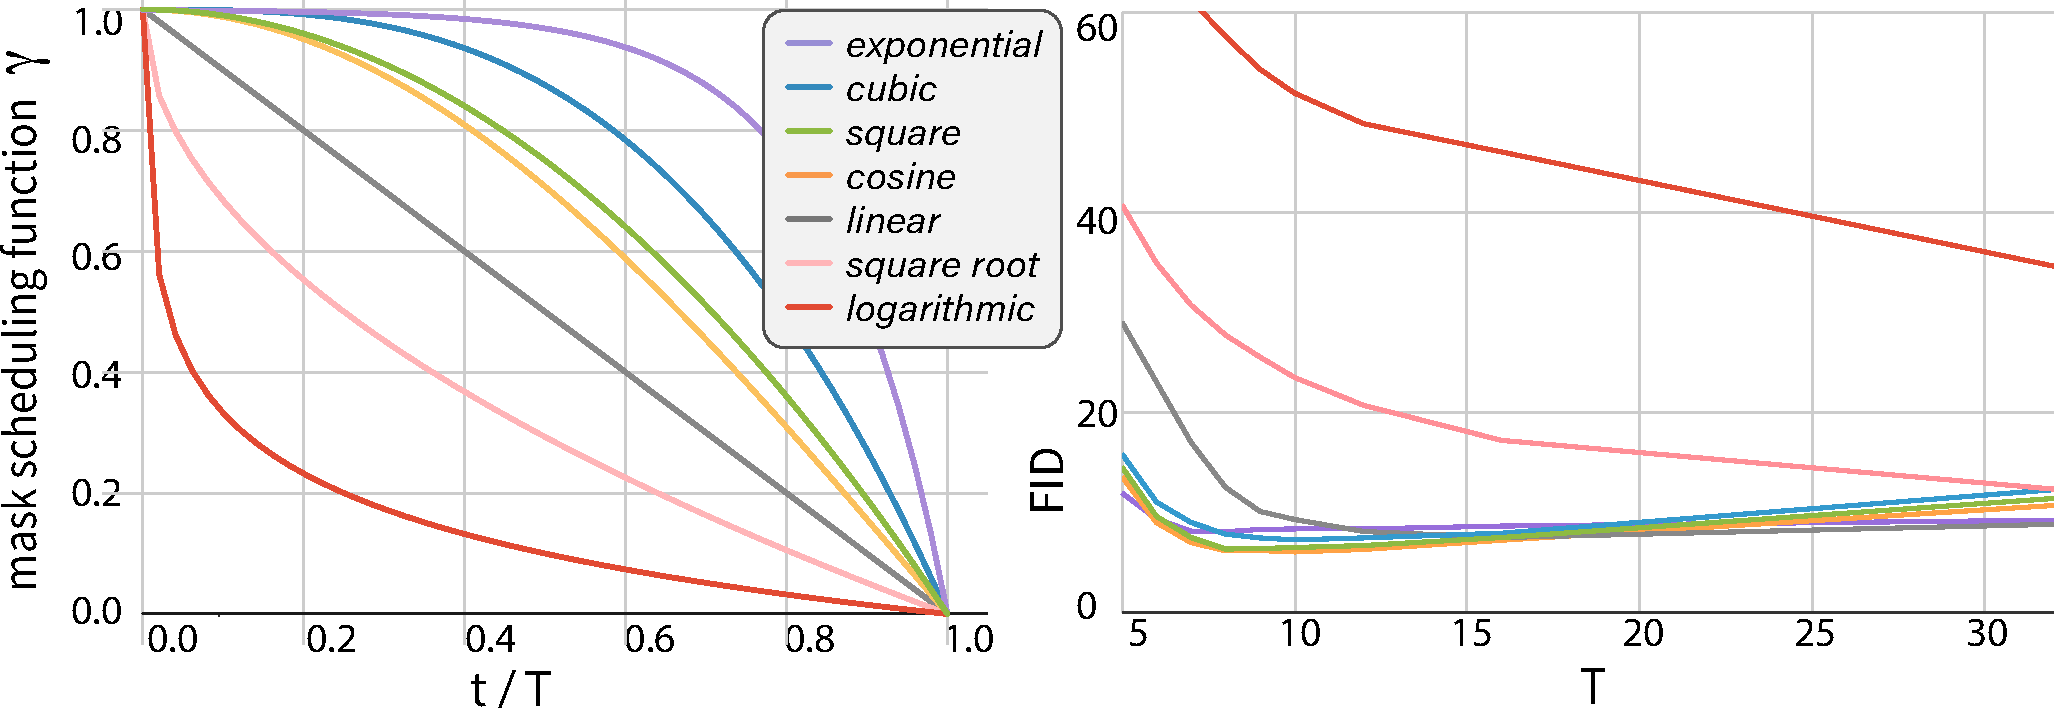
\includegraphics[width=1.\linewidth]{figures/scheduling_func.pdf}
    \vspace{-6mm}
    \caption{\textbf{掩码调度函数的选择} $\gamma (\frac{t}{T})$ 和 \textbf{迭代次数 \textit{T}}。左图显示我们为 $\gamma$ 考虑的七个函数的可视化。右图显示模型的 FID 分数与解码迭代次数 $T$ 的关系曲线。在候选函数中，我们发现余弦函数实现了最佳的 FID。}
    \label{fig:scheduling}
    \vspace{-3mm}
\end{figure}

\noindent{\textbf{Iteration number.}}
We study the effect of the number of iterations ($T$) on our model by running all candidate masking functions with different $T$s. As shown in Figure~\ref{fig:scheduling}, under the same setting, more iterations are not necessarily better: as $T$ increases, aside from the logarithmic function which performs poorly throughout, all other functions hit a ``sweet spot" where the model's performance peaks before it worsens again. The sweet spot also gets ``delayed" as functions get less concave. As shown, among functions that achieve strong FIDs (\ie cosine, square, and linear), cosine not only has the strongest overall score, but also the earliest sweet spot at a total of $8$ to $12$ iterations.
We hypothesize that such sweet spots exist because too many iterations may discourage the model from keeping less confident predictions, which worsens the token diversity. We think further study on the masking design would be interesting for future work.
